\documentclass{article}

\usepackage[preprint]{neurips_2026}

\usepackage[utf8]{inputenc}
\usepackage[T1]{fontenc}
\usepackage[hypertexnames=false]{hyperref}
\usepackage{url}
\usepackage{booktabs}
\usepackage{amsmath}
\usepackage{amsfonts}
\usepackage{graphicx}
\usepackage{xcolor}
\usepackage{microtype}
\usepackage{algorithm}
\usepackage[noend]{algpseudocode}
\usepackage{tikz}
\usetikzlibrary{arrows.meta, positioning, calc}

\title{A Scaled-Down Reproduction of StemGen for Context-Aware Bass Stem Generation}

\author{%
  StemGen Reproduction Team (Group 58) \\
  ECE 228 Final Project \\
  \texttt{https://github.com/daw041/ECE228\_stemGen.git}
}

\begin{document}

\maketitle

\begin{abstract}
This project studies context-aware music stem generation. Given a music mixture with the target instrument removed, the goal is to generate a target bass stem that matches the rhythm, harmony, and structure of the context. We reproduce the main idea of StemGen in a smaller course-scale setting: waveform audio is converted into EnCodec residual vector quantization (RVQ) tokens, target tokens are randomly masked, and a non-autoregressive Transformer predicts the missing target tokens conditioned on context tokens and an instrument label. Our best audio-token experiment uses 1000 Slakh-style multitrack songs, 10 second fixed-stride windows, two EnCodec codebooks, token-cache precomputation, and H100 training. It reaches a best validation loss of 3.0279 and validation token accuracy of 0.572, improving over the 550-track cached baseline by 12.3\% relative loss and 5.1 accuracy points. Qualitative mel-spectrogram diagnostics show that codec reconstruction and partial-mask reconstruction preserve useful bass structure, while full 100\% mask generation remains the main bottleneck.
\end{abstract}

\section{Introduction}

Music stem generation asks a model to create one instrument part while listening to the rest of the song. This is harder than ordinary unconditional audio generation. A bass stem should not only sound like bass; it should also follow the beat, support the harmony, and enter or stop at musically reasonable times. This capability matters in practice: context-aware stem generation underpins tools for music co-creation, accompaniment and backing-track production, instrument-aware remixing, and data augmentation for source separation, all of which need a model that responds to an existing mix rather than generating in isolation. In this project, the input context is the mixture with the bass stem removed, and the output is the generated bass stem.

Our work is a paper-guided reproduction of StemGen \citep{stemgen}. The official repository provides examples and demo material but not a full training pipeline or released weights, so we implement a smaller version of the core audio-token idea. The final system uses EnCodec \citep{encodec} to discretize audio into RVQ tokens, trains a masked-token Transformer to predict target bass tokens, and decodes predicted tokens back to waveform audio.

The main contributions are:
\begin{itemize}
    \item We built an end-to-end context-to-bass audio-token pipeline with EnCodec tokenization, multi-codebook masked cross entropy, and iterative mask-predict decoding.
    \item We fixed several reproduction issues, especially inconsistent codebook handling, inactive target clips, and slow online tokenization.
    \item We ran controlled experiments from small baselines to 550-track and 1000-track cached H100 runs, showing clear improvement in validation loss and token accuracy.
    \item We used codec reconstruction, partial-mask reconstruction, full-mask generation, and mel-spectrogram diagnostics to separate what works from what still fails.
\end{itemize}

\section{Related Work}

Neural music generation has recently moved from symbolic note models to audio-token models. MusicGen \citep{musicgen} generates music from discrete audio tokens using a language-model style decoder. SoundStorm \citep{soundstorm} and MaskGIT \citep{maskgit} show that masked parallel token prediction can generate high-quality discrete sequences with fewer decoding steps than fully autoregressive models. StemGen \citep{stemgen} applies this general direction to musical stem generation: the model listens to context stems and predicts a target stem in audio-token space. A practical limitation of this line of work for reproduction is that the strongest systems rely on large models and proprietary data, and the official StemGen release ships demos but neither a full training pipeline nor pretrained weights; MusicGen and SoundStorm likewise target unconditional or text-conditioned generation rather than mixture-conditioned stem completion. Our contribution is to close this gap with a compact, fully specified, and reproducible implementation of the core context-to-stem masked-token recipe that runs at course scale, isolating which parts of the method survive aggressive downscaling.

Audio tokenization is a key component. EnCodec \citep{encodec} compresses waveform audio into discrete RVQ codebooks and reconstructs audio from those codes. This makes audio generation closer to language modeling, because the model predicts token classes instead of raw samples. However, more codebooks also make prediction harder, because each time frame has multiple discrete targets.

We also explored a MIDI branch inspired by symbolic music generation. MIDI is easier to inspect and edit, but mapping context audio to bass notes was not reliable in our experiments. Frame-level MIDI baselines with mel/chroma features, CRNNs, and HuBERT features improved activity detection only up to about 0.289 F1. Since the project goal is to reproduce StemGen's audio-token method, we treat the MIDI branch as an exploratory baseline and keep the final method focused on audio tokens.

\section{Method / Approach}

\subsection{Task formulation}

For each multitrack song, let $x^{\mathrm{bass}}$ be the target bass stem and $x^{\mathrm{ctx}}$ be the sum of all non-bass stems. The model receives $x^{\mathrm{ctx}}$ and an instrument condition $c=\mathrm{bass}$, and predicts the target stem:
\begin{equation}
    \hat{x}^{\mathrm{bass}} = f_\theta(x^{\mathrm{ctx}}, c).
\end{equation}
Instead of predicting waveform samples directly, both context and target audio are converted to EnCodec tokens:
\begin{equation}
    z^{\mathrm{ctx}}, z^{\mathrm{bass}} = \mathrm{EncodecEncode}(x^{\mathrm{ctx}}, x^{\mathrm{bass}}),
\end{equation}
where $z \in \{0,\ldots,1023\}^{K \times T}$, $K=2$ is the number of RVQ codebooks, and $T$ is the token sequence length for a 10 second clip. The 24~kHz EnCodec model uses a 320-sample frame hop, so it emits $24000/320 = 75$ frames per second and a 10 second clip yields $T \approx 750$ tokens per codebook; the model allocates a maximum sequence length of $T_{\max}=1024$ to leave headroom above this value.

\subsection{Audio-token pipeline}

Figure~\ref{fig:pipeline} summarizes the implemented pipeline. We use 24 kHz EnCodec, 1.5 kbps bandwidth, two RVQ codebooks, and 10 second clips. The context is always visible. The target token sequence is partially or fully masked, and the model predicts the original target tokens.

\begin{figure}[t]
    \centering
    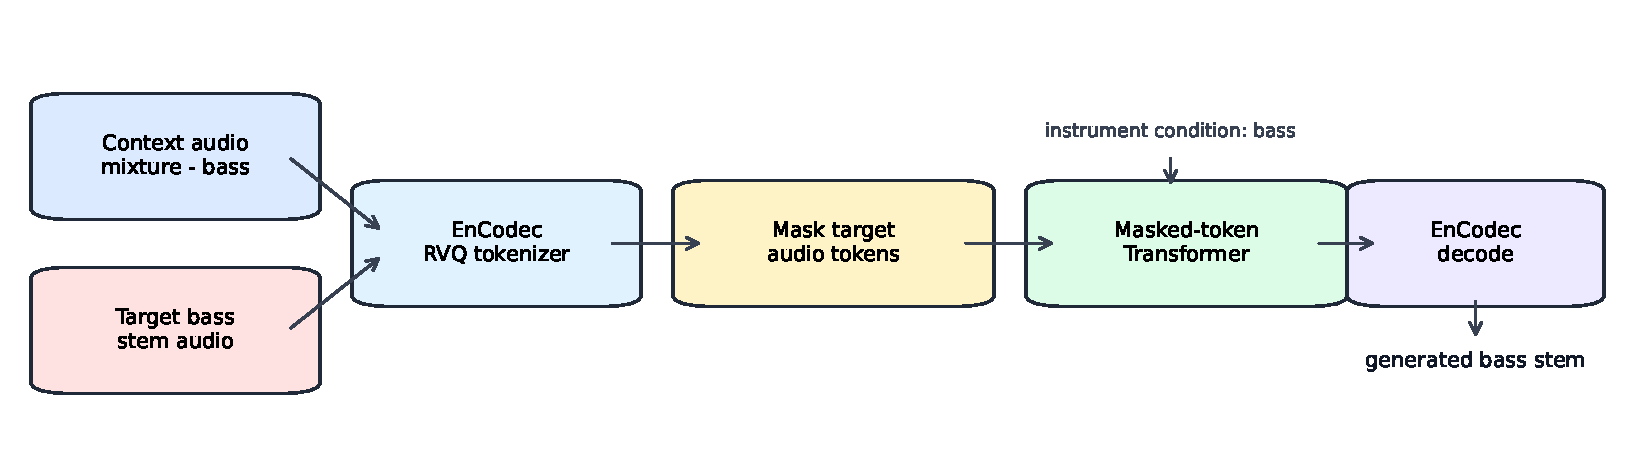
\includegraphics[width=\linewidth]{figures/pipeline.pdf}
    \caption{Audio-token reproduction pipeline. Context audio is the mixture without bass. Target bass audio is tokenized, masked, predicted by a Transformer, and decoded back to waveform audio.}
    \label{fig:pipeline}
\end{figure}

\begin{figure}[t]
    \centering
    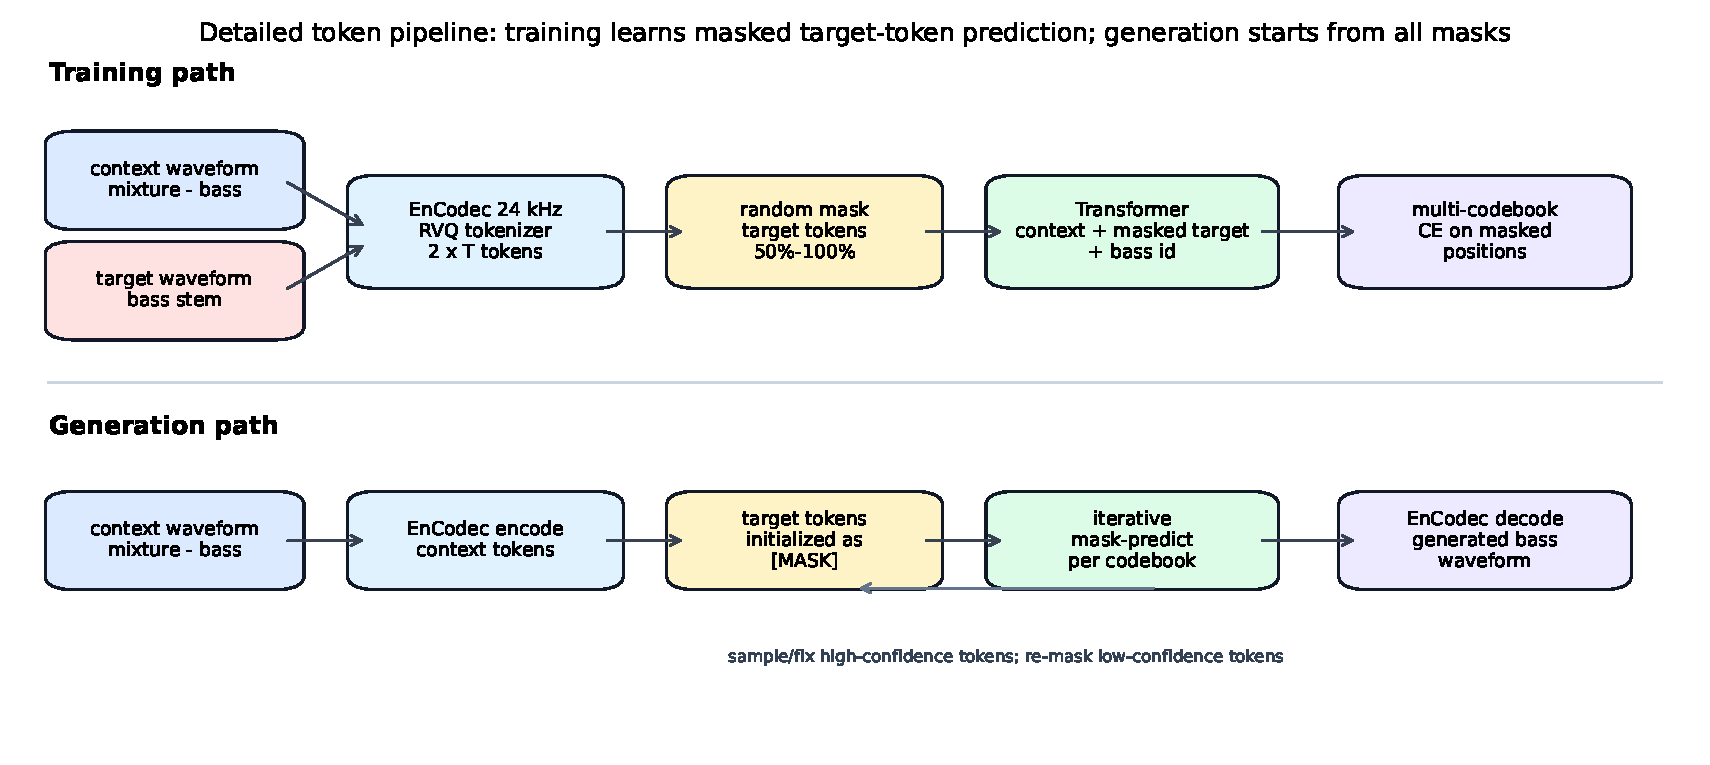
\includegraphics[width=\linewidth]{figures/detailed_pipeline.pdf}
    \caption{Detailed training and generation paths. During training, the model sees context tokens and a partially masked target token sequence. During generation, the target starts fully masked and is filled by iterative mask-predict decoding.}
    \label{fig:detailed_pipeline}
\end{figure}

\subsection{EnCodec RVQ tokenization}

EnCodec is a pretrained neural audio codec. It has an encoder that maps waveform audio into discrete residual vector quantization (RVQ) codes and a decoder that maps those codes back to waveform audio. In this project, EnCodec is not trained by us; it is used as a fixed tokenizer and detokenizer. This design changes the learning problem from raw waveform regression to discrete token classification.

For a 10 second clip, the codec produces a tensor with shape $[K,T]$, where $K$ is the number of RVQ codebooks and $T$ is the number of codec time frames. We use $K=2$. Each codebook has a vocabulary of 1024 entries, so each token is an integer in $[0,1023]$. The first codebook carries the coarse audio content, while the second codebook stores residual detail. The special mask token is assigned id 1024 and is only used by the Transformer, not by EnCodec.

The codebook count has to stay consistent through the whole pipeline. During encoding, both context and target waveforms become two-codebook token tensors. During training, the loss is computed for both codebooks. During decoding, the generated token tensor must also contain exactly two codebooks. We found this detail important because padding a missing codebook with token 0 is wrong: token 0 is a real codec codeword, not silence.

\subsection{Masked-token Transformer}

The model follows a two-stream design. Context tokens and target tokens have separate token embeddings. For each time step, embeddings from the two codebooks are summed inside each stream. An instrument embedding is repeated over time and concatenated with the context and target representations:
\begin{equation}
    h_t = W_f [e_{\mathrm{ctx}}(z^{\mathrm{ctx}}_t), e_{\mathrm{tar}}(\tilde{z}^{\mathrm{bass}}_t), e_{\mathrm{inst}}(c)] + p_t,
\end{equation}
where $\tilde{z}^{\mathrm{bass}}$ is the masked target sequence and $p_t$ is a learned positional embedding. A Transformer encoder maps $h_{1:T}$ to hidden states. Separate output heads predict each RVQ codebook:
\begin{equation}
    p_\theta(z^{\mathrm{bass}}_{k,t} \mid z^{\mathrm{ctx}}, \tilde{z}^{\mathrm{bass}}, c)
    = \mathrm{softmax}(W_k h_t).
\end{equation}

The final model uses 8 Transformer layers, hidden size $d=512$, 8 attention heads, feed-forward size 2048, dropout 0.1, and vocabulary size 1024 plus one mask token. Token embeddings are shared across codebook levels within each stream: for a given time step $t$, the representation is formed by summing the $d$-dimensional embeddings of all $K$ codebook tokens at that position rather than using separate per-codebook embedding tables, so each stream produces one $512$-dimensional vector per frame. The instrument condition is mapped by a separate embedding table over $6$ instrument classes to a $64$-dimensional vector $e_{\mathrm{inst}}(c)$ and broadcast over time. The context stream embedding $e_{\mathrm{ctx}}$ ($512$), target stream embedding $e_{\mathrm{tar}}$ ($512$), and instrument embedding $e_{\mathrm{inst}}$ ($64$) are concatenated along the feature dimension to a $512+512+64=1088$ dimensional vector and projected back to the model dimension $d=512$ via a learned linear layer $W_f \in \mathbb{R}^{512 \times 1088}$ before positional encoding is added. We use concatenation-then-projection rather than simple addition so the model can learn an asymmetric weighting of the three streams instead of forcing them onto a shared subspace. Positional encoding is a learned parameter matrix of shape $[1, T_{\max}, d]$ with $T_{\max}=1024$ rather than a fixed sinusoidal encoding. The Transformer uses Pre-LayerNorm (norm-first) and GELU activations. Output heads for each codebook are independent linear layers mapping $\mathbb{R}^d \to \mathbb{R}^{1024}$, with no weight sharing between codebooks. An optional frame-level activity head is implemented but disabled in the final audio-token model. The total parameter count is approximately 28.4 million. Figure~\ref{fig:arch} traces the data flow through the two streams, the conditioning embedding, the fusion projection, and the per-codebook output heads.

\begin{figure}[t]
    \centering
    \resizebox{\linewidth}{!}{%
    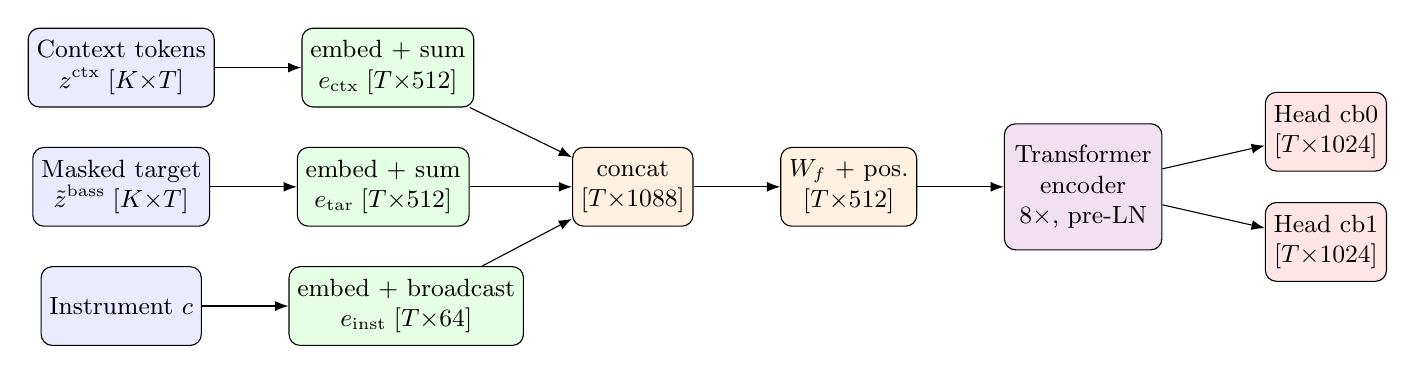
\begin{tikzpicture}[
      font=\small, >=Latex, node distance=5mm and 11mm,
      box/.style={draw, rounded corners, align=center, minimum height=10mm, inner sep=3pt},
      inp/.style={box, fill=blue!8},
      emb/.style={box, fill=green!10},
      op/.style={box, fill=orange!12},
      tf/.style={box, fill=violet!12, minimum height=16mm, minimum width=20mm},
      head/.style={box, fill=red!10},
    ]
      \node[inp] (ctx) {Context tokens\\ $z^{\mathrm{ctx}}\;[K{\times}T]$};
      \node[inp, below=of ctx] (tar) {Masked target\\ $\tilde z^{\mathrm{bass}}\;[K{\times}T]$};
      \node[inp, below=of tar] (inst) {Instrument $c$};

      \node[emb, right=of ctx]  (ectx)  {embed $+$ sum\\ $e_{\mathrm{ctx}}\;[T{\times}512]$};
      \node[emb, right=of tar]  (etar)  {embed $+$ sum\\ $e_{\mathrm{tar}}\;[T{\times}512]$};
      \node[emb, right=of inst] (einst) {embed $+$ broadcast\\ $e_{\mathrm{inst}}\;[T{\times}64]$};

      \node[op, right=13mm of etar] (concat) {concat\\ $[T{\times}1088]$};
      \node[op, right=of concat] (proj) {$W_f$ $+$ pos.\\ $[T{\times}512]$};
      \node[tf, right=of proj] (trans) {Transformer\\ encoder\\ $8\times$, pre-LN};

      \node[head, right=13mm of trans, yshift=7mm]  (h0) {Head cb0\\ $[T{\times}1024]$};
      \node[head, right=13mm of trans, yshift=-7mm] (h1) {Head cb1\\ $[T{\times}1024]$};

      \draw[->] (ctx)  -- (ectx);
      \draw[->] (tar)  -- (etar);
      \draw[->] (inst) -- (einst);
      \draw[->] (ectx)  -- (concat);
      \draw[->] (etar)  -- (concat);
      \draw[->] (einst) -- (concat);
      \draw[->] (concat) -- (proj);
      \draw[->] (proj) -- (trans);
      \draw[->] (trans) -- (h0);
      \draw[->] (trans) -- (h1);
    \end{tikzpicture}}
    \caption{Two-stream masked-token Transformer. The context and (masked) target token streams are each embedded and summed across the $K=2$ codebooks into $512$-dimensional per-frame vectors; the instrument embedding is broadcast over time. The three are concatenated to $1088$ dimensions, projected back to $d=512$ by $W_f$, given learned positional encodings, and passed through an 8-layer pre-LN Transformer. Independent linear heads predict the $1024$-way token distribution for each codebook.}
    \label{fig:arch}
\end{figure}

\subsection{Training objective}

During training, a target mask ratio is sampled uniformly between 0.50 and 1.00 per batch. The mask is applied at the \emph{frame} level: a single binary mask over time positions is drawn and applied identically across all codebooks, so the same time steps are masked in both codebook sequences. This is important for coherence: revealing a time step in codebook 0 while masking it in codebook 1 would create an inconsistent input that does not occur at generation time. The model is trained with masked cross entropy over all masked positions and both codebooks:
\begin{equation}
    \mathcal{L}
    =
    \sum_{k=1}^{K}
    \sum_{t \in \mathcal{M}_k}
    \mathrm{CE}
    \left(
    p_\theta(z^{\mathrm{bass}}_{k,t}),
    z^{\mathrm{bass}}_{k,t}
    \right).
\end{equation}
This was an important cleanup step. Earlier versions only handled one codebook or padded missing codebooks with token 0 during decoding, which produced poor audio artifacts.

The training path is therefore:
\begin{enumerate}
    \item Build $x^{\mathrm{ctx}}$ by summing all non-bass stems and take $x^{\mathrm{bass}}$ as the target.
    \item Encode both waveforms with EnCodec to get $z^{\mathrm{ctx}}, z^{\mathrm{bass}} \in \{0,\ldots,1023\}^{2 \times T}$.
    \item Randomly replace 50--100\% of target tokens with the mask token 1024.
    \item Feed context tokens, masked target tokens, and the bass instrument id into the Transformer.
    \item Compute cross entropy only at masked target positions, separately for each codebook, and sum the losses.
\end{enumerate}

Algorithm~\ref{alg:train} states one training step precisely. The key design choice is that a single binary mask is drawn over the $T$ time positions and applied identically to both codebooks, so the model never sees the inconsistent situation of a frame revealed in one codebook but masked in the other---a situation that cannot occur at generation time.

\begin{algorithm}[t]
\caption{Masked audio-token training step}
\label{alg:train}
\begin{algorithmic}[1]
\Require context tokens $z^{\mathrm{ctx}}\!\in\!\{0,\ldots,1023\}^{K\times T}$, target tokens $z^{\mathrm{bass}}\!\in\!\{0,\ldots,1023\}^{K\times T}$, instrument $c$, model $f_\theta$
\State sample mask ratio $r \sim \mathcal{U}(0.50, 1.00)$
\State draw frame mask $m \in \{0,1\}^{T}$ with $\Pr[m_t=1]=r$ \Comment{shared across all $K$ codebooks}
\State $\tilde{z}^{\mathrm{bass}}_{k,t} \gets 1024$ if $m_t=1$ else $z^{\mathrm{bass}}_{k,t}$, for all $k,t$ \Comment{insert mask token}
\State $\{p_\theta(\cdot\mid k,t)\}_{k,t} \gets f_\theta(z^{\mathrm{ctx}}, \tilde{z}^{\mathrm{bass}}, c)$
\State $\mathcal{L} \gets \sum_{k=1}^{K}\sum_{t:\,m_t=1} \mathrm{CE}\!\left(p_\theta(\cdot\mid k,t),\, z^{\mathrm{bass}}_{k,t}\right)$ \Comment{equal codebook weights $[1,1]$}
\State update $\theta$ with AdamW on $\nabla_\theta \mathcal{L}$ under AMP, gradient clipped to norm $1.0$
\end{algorithmic}
\end{algorithm}

\subsection{Iterative generation and diagnostics}

For full generation, target tokens start as all masks. The model predicts a token distribution, keeps high-confidence predictions, re-masks the rest, and repeats this process codebook by codebook. In our implementation, codebook 0 is generated first because it represents coarse structure. Later codebooks are generated after earlier codebooks are available, so the residual prediction can condition on the coarse prediction.

The generation loop is:
\begin{enumerate}
    \item Encode the context waveform into context tokens.
    \item Initialize all target tokens as $[\mathrm{MASK}]$.
    \item For each codebook, run several mask-predict iterations.
    \item At each iteration, predict logits for currently masked positions, apply temperature or top-$k$ sampling if enabled, and fill candidate tokens.
    \item Rank predictions by confidence, keep a growing fraction of high-confidence tokens, and set low-confidence tokens back to $[\mathrm{MASK}]$ for the next iteration.
    \item After all codebooks are filled, decode the generated token tensor with EnCodec to obtain the bass waveform.
\end{enumerate}

At each iteration, the confidence score used to rank which tokens to keep is:
\begin{equation}
    s_{t} = \max_v\, p_\theta(z^{\mathrm{bass}}_{k,t} = v) + \lambda \cdot b_t,
\end{equation}
where $b_t = (T - t) / T$ is a causal position bias that favors fixing earlier time positions first, and $\lambda = 0.1$ controls its strength. At iteration $i$ of $N_k$ total iterations for codebook $k$, let $B$ be the number of positions still masked in that codebook; the schedule commits the top-scoring
\begin{equation}
    \max\!\left(1,\; \left\lfloor B \cdot r \cdot \frac{i+1}{N_k} \right\rfloor\right)
\end{equation}
positions and re-masks the rest, with a base keep ratio $r = 0.25$. We use a deeper schedule for the coarse codebook, $N_0 = 32$ and $N_1 = 16$, since codebook~0 carries the structure that the residual codebook conditions on. This progressive reveal means that in early iterations only a small fraction of high-confidence positions are committed, leaving uncertain positions open for revision in later iterations. Sampling defaults to temperature $1.0$ with multinomial draws and optional top-$k$ truncation; greedy decoding is also supported.

Algorithm~\ref{alg:gen} states the full decoding procedure, and Figure~\ref{fig:schedule} illustrates the progressive reveal as a storyboard.

\begin{algorithm}[t]
\caption{Iterative coarse-to-fine mask-predict generation}
\label{alg:gen}
\begin{algorithmic}[1]
\Require context tokens $z^{\mathrm{ctx}}$, instrument $c$, model $f_\theta$, iterations $\{N_k\}$, keep ratio $r$, bias $\lambda$
\State initialize all target tokens $\hat{z}_{k,t} \gets 1024$ for every $k,t$
\For{codebook $k = 0$ to $K-1$} \Comment{coarse to fine}
  \For{iteration $i = 0$ to $N_k-1$}
    \State $p_\theta \gets f_\theta(z^{\mathrm{ctx}}, \hat{z}, c)$; restrict attention to codebook $k$
    \State sample/argmax a candidate $v_t$ for each masked position $t$ from $p_\theta(\cdot\mid k,t)$
    \State score $s_t \gets \max_v p_\theta(z_{k,t}=v) + \lambda (T-t)/T$
    \State keep the top $\max(1, \lfloor B\, r\,(i{+}1)/N_k\rfloor)$ positions by $s_t$; set $\hat{z}_{k,t}\!\gets\! v_t$ there
    \State re-mask all other positions of codebook $k$
  \EndFor
\EndFor
\State \Return EnCodec decode of $\hat{z}$ as the bass waveform
\end{algorithmic}
\end{algorithm}

\begin{figure}[t]
    \centering
    \newcommand{\tokrow}[4]{%
      \foreach \i in {1,...,#3}{%
        \pgfmathtruncatemacro{\isfix}{\i < #4 + 0.5 ? 1 : 0}%
        \ifnum\isfix=1\relax
          \node[fix] at ({#1+(\i-1)*0.46},#2) {};%
        \else
          \node[mask] at ({#1+(\i-1)*0.46},#2) {};%
        \fi
      }%
    }
    \resizebox{\linewidth}{!}{%
    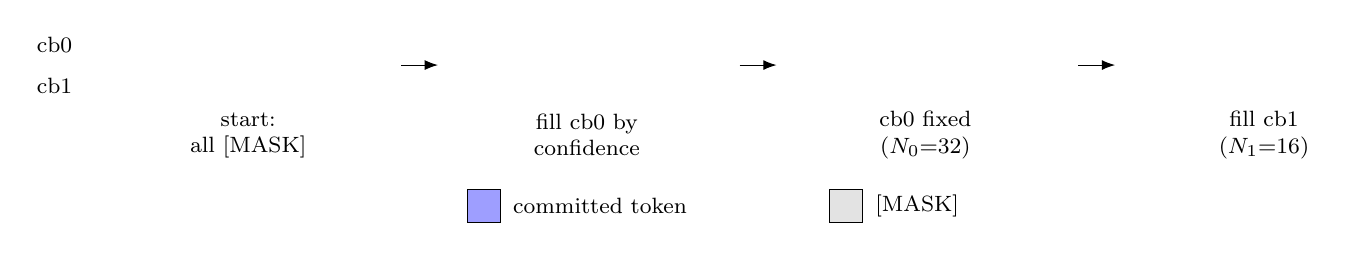
\begin{tikzpicture}[font=\footnotesize, >=Latex,
      cell/.style={draw, minimum size=4.2mm, inner sep=0pt},
      mask/.style={cell, fill=gray!22},
      fix/.style={cell, fill=blue!38},
    ]
      \node at (-0.85,0) {cb0};
      \node at (-0.85,-0.52) {cb1};
      % stage A: all masked
      \tokrow{0}{0}{8}{0}      \tokrow{0}{-0.52}{8}{0}
      % stage B: cb0 partly committed
      \tokrow{4.3}{0}{8}{3}    \tokrow{4.3}{-0.52}{8}{0}
      % stage C: cb0 done
      \tokrow{8.6}{0}{8}{8}    \tokrow{8.6}{-0.52}{8}{0}
      % stage D: cb1 done
      \tokrow{12.9}{0}{8}{8}   \tokrow{12.9}{-0.52}{8}{8}
      % stage labels
      \node[align=center] at (1.61,-1.15)  {start:\\ all [MASK]};
      \node[align=center] at (5.91,-1.15)  {fill cb0 by\\ confidence};
      \node[align=center] at (10.21,-1.15) {cb0 fixed\\ ($N_0{=}32$)};
      \node[align=center] at (14.51,-1.15) {fill cb1\\ ($N_1{=}16$)};
      % transition arrows
      \draw[->] (3.55,-0.26)  -- (4.02,-0.26);
      \draw[->] (7.85,-0.26)  -- (8.32,-0.26);
      \draw[->] (12.15,-0.26) -- (12.62,-0.26);
      % legend
      \node[fix]  at (4.6,-2.05) {}; \node[right] at (4.85,-2.05) {committed token};
      \node[mask] at (9.2,-2.05) {}; \node[right] at (9.45,-2.05) {[MASK]};
    \end{tikzpicture}}
    \caption{Coarse-to-fine mask-predict generation. The target starts as all mask tokens. Codebook~0 is filled first over $N_0=32$ iterations, committing the most confident positions at each step (the causal bias favors earlier time positions, drawn as a left-to-right fill); once codebook~0 is fixed, codebook~1 is filled over $N_1=16$ iterations conditioned on it. The decoded token tensor is then passed to EnCodec.}
    \label{fig:schedule}
\end{figure}

We evaluate three levels:
\begin{itemize}
    \item Codec reconstruction: encode and decode the real target stem to check whether the tokenizer setting is usable.
    \item Partial-mask reconstruction: reveal part of the target tokens and predict the masked part.
    \item Full-mask generation: generate the entire target only from context and instrument condition.
\end{itemize}
This diagnostic split is useful because a model can learn local token reconstruction while still failing at full context-to-stem generation.

\subsection{Hyperparameter summary}

Table~\ref{tab:hparams} consolidates the model, codec, training, and generation settings of the final system for reproducibility.

\begin{table}[t]
\centering
\caption{Configuration of the final audio-token system.}
\label{tab:hparams}
\small
\begin{tabular}{llll}
\toprule
\multicolumn{2}{l}{\textbf{Model / codec}} & \multicolumn{2}{l}{\textbf{Training / generation}} \\
\midrule
Transformer layers & 8 & Optimizer & AdamW \\
Hidden size $d$ & 512 & Learning rate & $3\times10^{-4}$ \\
Attention heads & 8 & $\beta_1,\beta_2$ & $0.9, 0.999$ \\
Feed-forward size & 2048 & Weight decay & $10^{-5}$ \\
Activation / norm & GELU / pre-LN & Batch size & 64 \\
Dropout & 0.1 & Grad clip (norm) & 1.0 \\
Positional enc. & learned, $T_{\max}{=}1024$ & Precision & AMP (fp16) \\
Instrument embed dim & 64 ($6$ classes) & Mask ratio $r$ & $\mathcal{U}(0.5,1.0)$ \\
Output heads & per-codebook & Codebook weights & $[1.0, 1.0]$ \\
Parameters & $\approx$28.4\,M & Early stop & patience 12, $\delta{=}0.005$ \\
\midrule
Codec & EnCodec 24\,kHz & Gen.\ iterations $N_0,N_1$ & 32, 16 \\
Bandwidth & 1.5\,kbps & Keep ratio $r$ & 0.25 \\
Codebooks $K$ & 2 ($\times$1024) & Causal bias $\lambda$ & 0.1 \\
Frame rate & 75\,Hz ($T{\approx}750$) & Sampling & temp.\ 1.0, multinomial \\
\bottomrule
\end{tabular}
\end{table}

\section{Results \& Analysis}

\subsection{Dataset and implementation details}

The data is a Slakh-style multitrack subset \citep{slakh}. We use bass as the target instrument. The context is the sum of all non-bass stems. Audio is resampled to 24 kHz and cut into 10 second clips. In later experiments, clips with weak or inactive bass are filtered by target activity so that validation accuracy is not inflated by silent examples.

Training uses AdamW with a constant learning rate $3\times 10^{-4}$, momentum parameters $\beta = (0.9, 0.999)$, weight decay $10^{-5}$, batch size 64, gradient clipping at norm $1.0$, and mixed-precision training (AMP). Early stopping monitors validation loss with patience 12 epochs and minimum improvement threshold $\delta = 0.005$. Codebook losses are weighted equally at $[1.0, 1.0]$. Token-cache precomputation was important for training efficiency: instead of running EnCodec online during every training epoch, we store context and target tokens in shards and train directly from token files.

We report \emph{masked token accuracy}: at the masked target positions, the fraction of positions where the model's top-1 prediction equals the ground-truth EnCodec token, averaged over the two codebooks. The 1000-track run uses a deterministic 80/20 train/validation split over fixed non-overlapping windows, so validation accuracy is comparable across epochs and runs rather than depending on a random crop.

For the final 1000-track fixed-stride cached run, the token cache contains 18,361 training clips and 4,567 validation clips after inactive bass filtering (approximately an 80/20 split). A clip is considered inactive and filtered if the target bass waveform energy falls below a threshold, preventing the model from overfitting to silent frames and inflating validation accuracy. The filtering removed 2,060 training candidates and 527 validation candidates from the raw stride-10 windows (roughly 10\% of each split).

As a reference point, a trivial random-token baseline that predicts each of the 1024 token classes uniformly at random would achieve an expected accuracy of $1/1024 \approx 0.10\%$. A majority-class baseline that always predicts the most frequent token would also perform near chance because codec token distributions are approximately uniform across the vocabulary. The model's best validation accuracy of 57.2\% therefore represents substantial learned structure rather than label imbalance. An upper bound for the token prediction task is codec reconstruction accuracy: encoding the ground-truth bass waveform with EnCodec and decoding it back recovers audio that is perceptually close to the original, confirming that the tokenizer setting is not the bottleneck.

\begin{figure}[t]
    \centering
    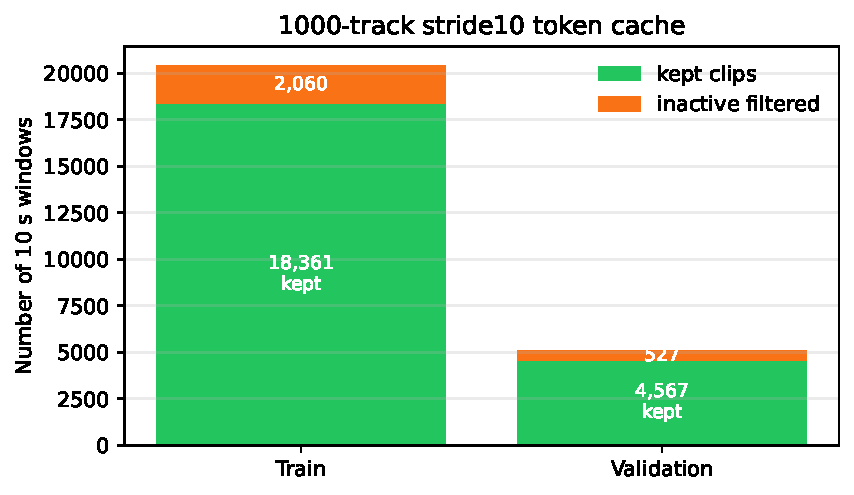
\includegraphics[width=0.95\linewidth]{figures/cache_filtering.pdf}
    \caption{Final 1000-track fixed-stride cache statistics. Inactive bass windows are filtered before training and validation.}
    \label{fig:cache}
\end{figure}

\subsection{Main quantitative results}

Table~\ref{tab:main_results} shows the main audio-token experiments. The strongest run is the 1000-track fixed-stride cached experiment. It uses non-overlapping 10 second windows, filters inactive target clips, and warm-starts from the 550-track checkpoint.

\begin{table}[t]
\centering
\caption{Main audio-token validation results. Accuracy is masked token accuracy averaged across codebooks when applicable.}
\label{tab:main_results}
\small
\begin{tabular}{lrlrr}
\toprule
Run & Clips & Sampling & Val loss & Val acc \\
\midrule
1cb, 315 tracks & -- & random 4 s & -- & 0.280 \\
2cb, 200 tracks & 1,197 & random 10 s & 6.0700 & 0.294 \\
2cb, 550 tracks & 3,262 & random 10 s & 3.6500 & 0.518 \\
2cb, 550 cached & 26,400 & cached clips & 3.4507 & 0.521 \\
2cb, 1000 stride10 cached & 22,928 & fixed 10 s stride & \textbf{3.0279} & \textbf{0.572} \\
\bottomrule
\end{tabular}
\end{table}

\begin{figure}[t]
    \centering
    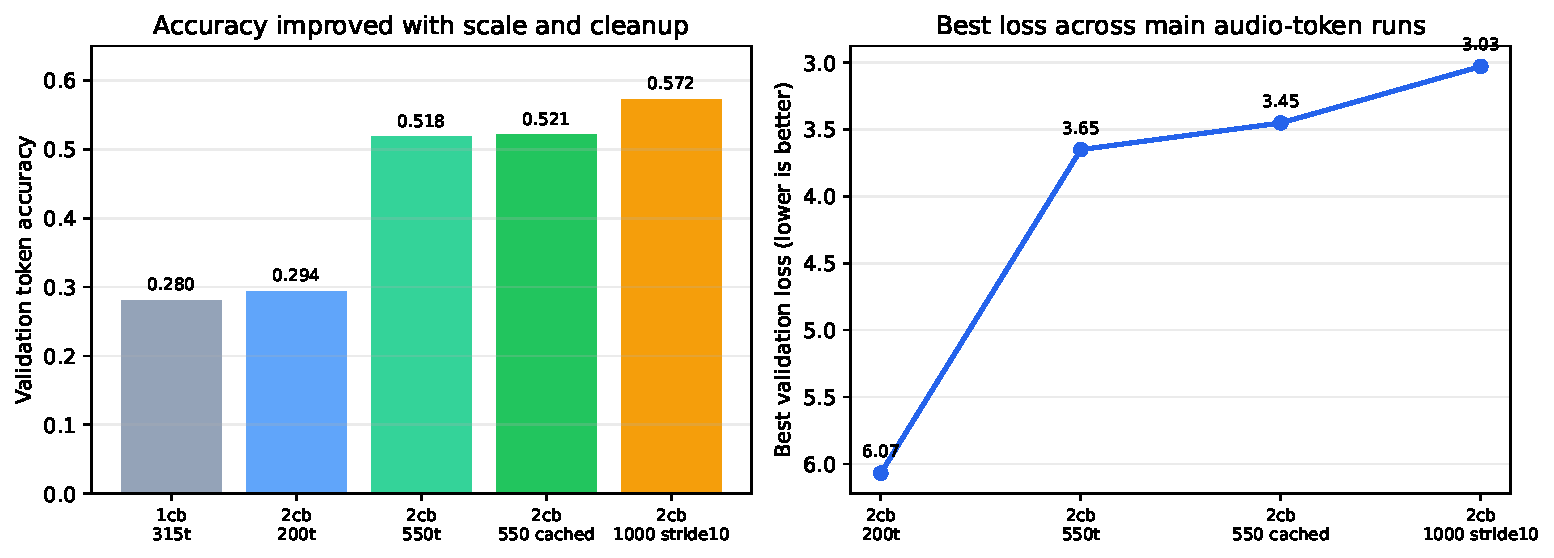
\includegraphics[width=\linewidth]{figures/results_summary.pdf}
    \caption{Validation accuracy and loss across the main audio-token runs. The final 1000-track stride10 cached run gives the best quantitative result.}
    \label{fig:results}
\end{figure}

The improvement from the 550 cached run to the 1000 stride10 cached run is meaningful. Best validation loss decreases from 3.4507 to 3.0279, a 12.3\% relative reduction. Validation accuracy increases from 0.521 to 0.572. The best epoch also moves from 56 to 19, which suggests that warm start plus cleaner fixed-stride data helped convergence.

The trend across experiments also shows why we did not report only one final number. The 200-track run already proves that the two-codebook setting is trainable, but its validation accuracy is still close to 0.29, and it early-stopped at epoch 226 (best validation at epoch 176). Scaling to 550 tracks gives the largest jump, from 0.294 to about 0.52, which means the model needs broader musical coverage to learn the mapping from context to bass tokens; notably the 550-track run ran the full 400 epochs without triggering early stopping and was still improving at the end (best at epoch 353), which directly motivated the move to token caching so that longer, larger-scale runs became affordable. The cached 550-track run is only slightly better in accuracy than the non-cached 550-track run, but it is much more practical because the GPU is no longer waiting for repeated EnCodec encoding. The final 1000-track run improves quality by changing the data distribution, not by simply adding more overlapping clips. It has fewer total clips than the cached 550 run, but the clips come from more songs and use fixed non-overlapping windows.

\subsection{Codebook-level analysis}

The final 1000-track run reaches codebook accuracies of $[0.6727, 0.4715]$ at the best checkpoint. The first codebook is easier because it carries coarse audio structure (timing, energy envelope, low-frequency content). The second codebook adds residual detail and is harder. A 4-codebook experiment on 150 tracks failed badly: it early-stopped at epoch 162 with only 0.168 overall validation accuracy, well below even the 0.28 single-codebook baseline, so larger codebook capacity needs more data and probably a larger model before it helps rather than hurts.

This gap between codebooks is important for audio quality. Predicting the first codebook mostly gives rough timing, energy, and low-frequency structure. Predicting later codebooks improves detail and timbre, but the label space becomes harder because many residual tokens may be plausible for the same context. In other words, token accuracy is not a perfect audio metric. A wrong fine codebook token may be less harmful than a wrong coarse token, while a sequence of confident but temporally inconsistent coarse tokens can sound very bad. For this reason, we report codebook accuracy but also rely on mel diagnostics.

\subsection{Ablation-style observations}

Several engineering changes were necessary before the results became interpretable. Table~\ref{tab:ablation} summarizes the most important ones. These are not perfectly isolated ablations, because the project schedule did not allow rerunning every combination, but each change fixed a concrete failure mode observed during development.

\begin{table}[t]
\centering
\caption{Important implementation and data changes.}
\label{tab:ablation}
\small
\begin{tabular}{p{0.24\linewidth}p{0.33\linewidth}p{0.32\linewidth}}
\toprule
Change & Problem before the change & Effect on the project \\
\midrule
Aligned codebook count & Codec, trainer, and generator could disagree on the number of RVQ levels. & Made loss and decoding consistent across two codebooks. \\
Multi-codebook loss & Early training mainly optimized codebook 0. & Forced the model to learn both coarse and residual token streams. \\
Inactive clip filtering & Silent or weak bass clips could give misleadingly easy accuracy. & Made validation more related to real bass generation. \\
Token cache & Online EnCodec encoding was slow and wasted H100 time. & Enabled larger cached runs and faster iteration. \\
Fixed stride windows & Random windows created many highly overlapping clips. & Reduced redundancy and improved generalization in the 1000-track run. \\
\bottomrule
\end{tabular}
\end{table}

\subsection{Convergence analysis}

The training dynamics differ notably across runs. The 550-track cached run required 56 epochs to reach its best validation loss of 3.4507, while the 1000-track stride10 run warm-started from that checkpoint and reached its best loss of 3.0279 at only epoch 19 before early stopping triggered at epoch 31. This faster convergence has two explanations. First, warm-starting from a partially trained checkpoint skips the early noisy phase where the model learns basic codebook statistics. Second, the fixed-stride non-overlapping windows in the 1000-track run present a more uniform data distribution: each clip is seen roughly once per epoch, whereas random sampling in earlier runs could revisit the same audio region many times within one epoch, slowing generalization.

The final checkpoint at epoch 31 (loss 3.2979, accuracy 0.543) is worse than the best at epoch 19, confirming that the model did overfit slightly after epoch 19. The early stopping patience of 12 epochs with minimum delta 0.005 correctly identified this and halted training, preventing further degradation. This suggests that the optimal training regime for the current data scale sits around 20--25 epochs with warm start, and that further improvement would require either more data or model regularization rather than simply longer training.

\begin{figure}[H]
    \centering
    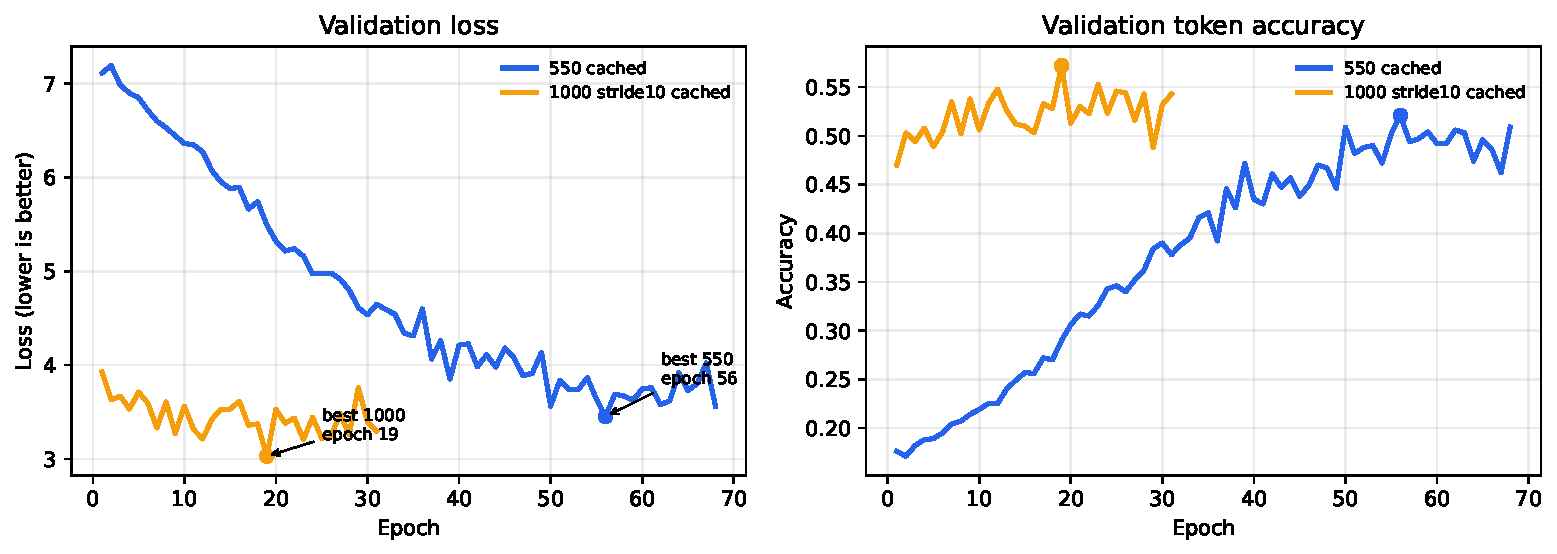
\includegraphics[width=\linewidth]{figures/training_curves.pdf}
    \caption{Validation loss and token accuracy curves for the two strongest cached audio-token runs. The 1000-track fixed-stride run starts from the 550-track checkpoint and reaches its best validation loss much earlier.}
    \label{fig:training_curves}
\end{figure}

\subsection{Qualitative analysis}

Figure~\ref{fig:mels} shows the mel-spectrogram diagnostic from the 550-track cached model. The exact audio quality is still not at paper level, but the diagnostic is useful. Codec reconstruction preserves the main target structure, so the tokenizer is not the main failure point. Partial-mask reconstruction produces more reasonable time-frequency structure than early noisy baselines. Full 100\% mask generation is weaker and can become noisy or misaligned.

\begin{figure}[H]
    \centering
    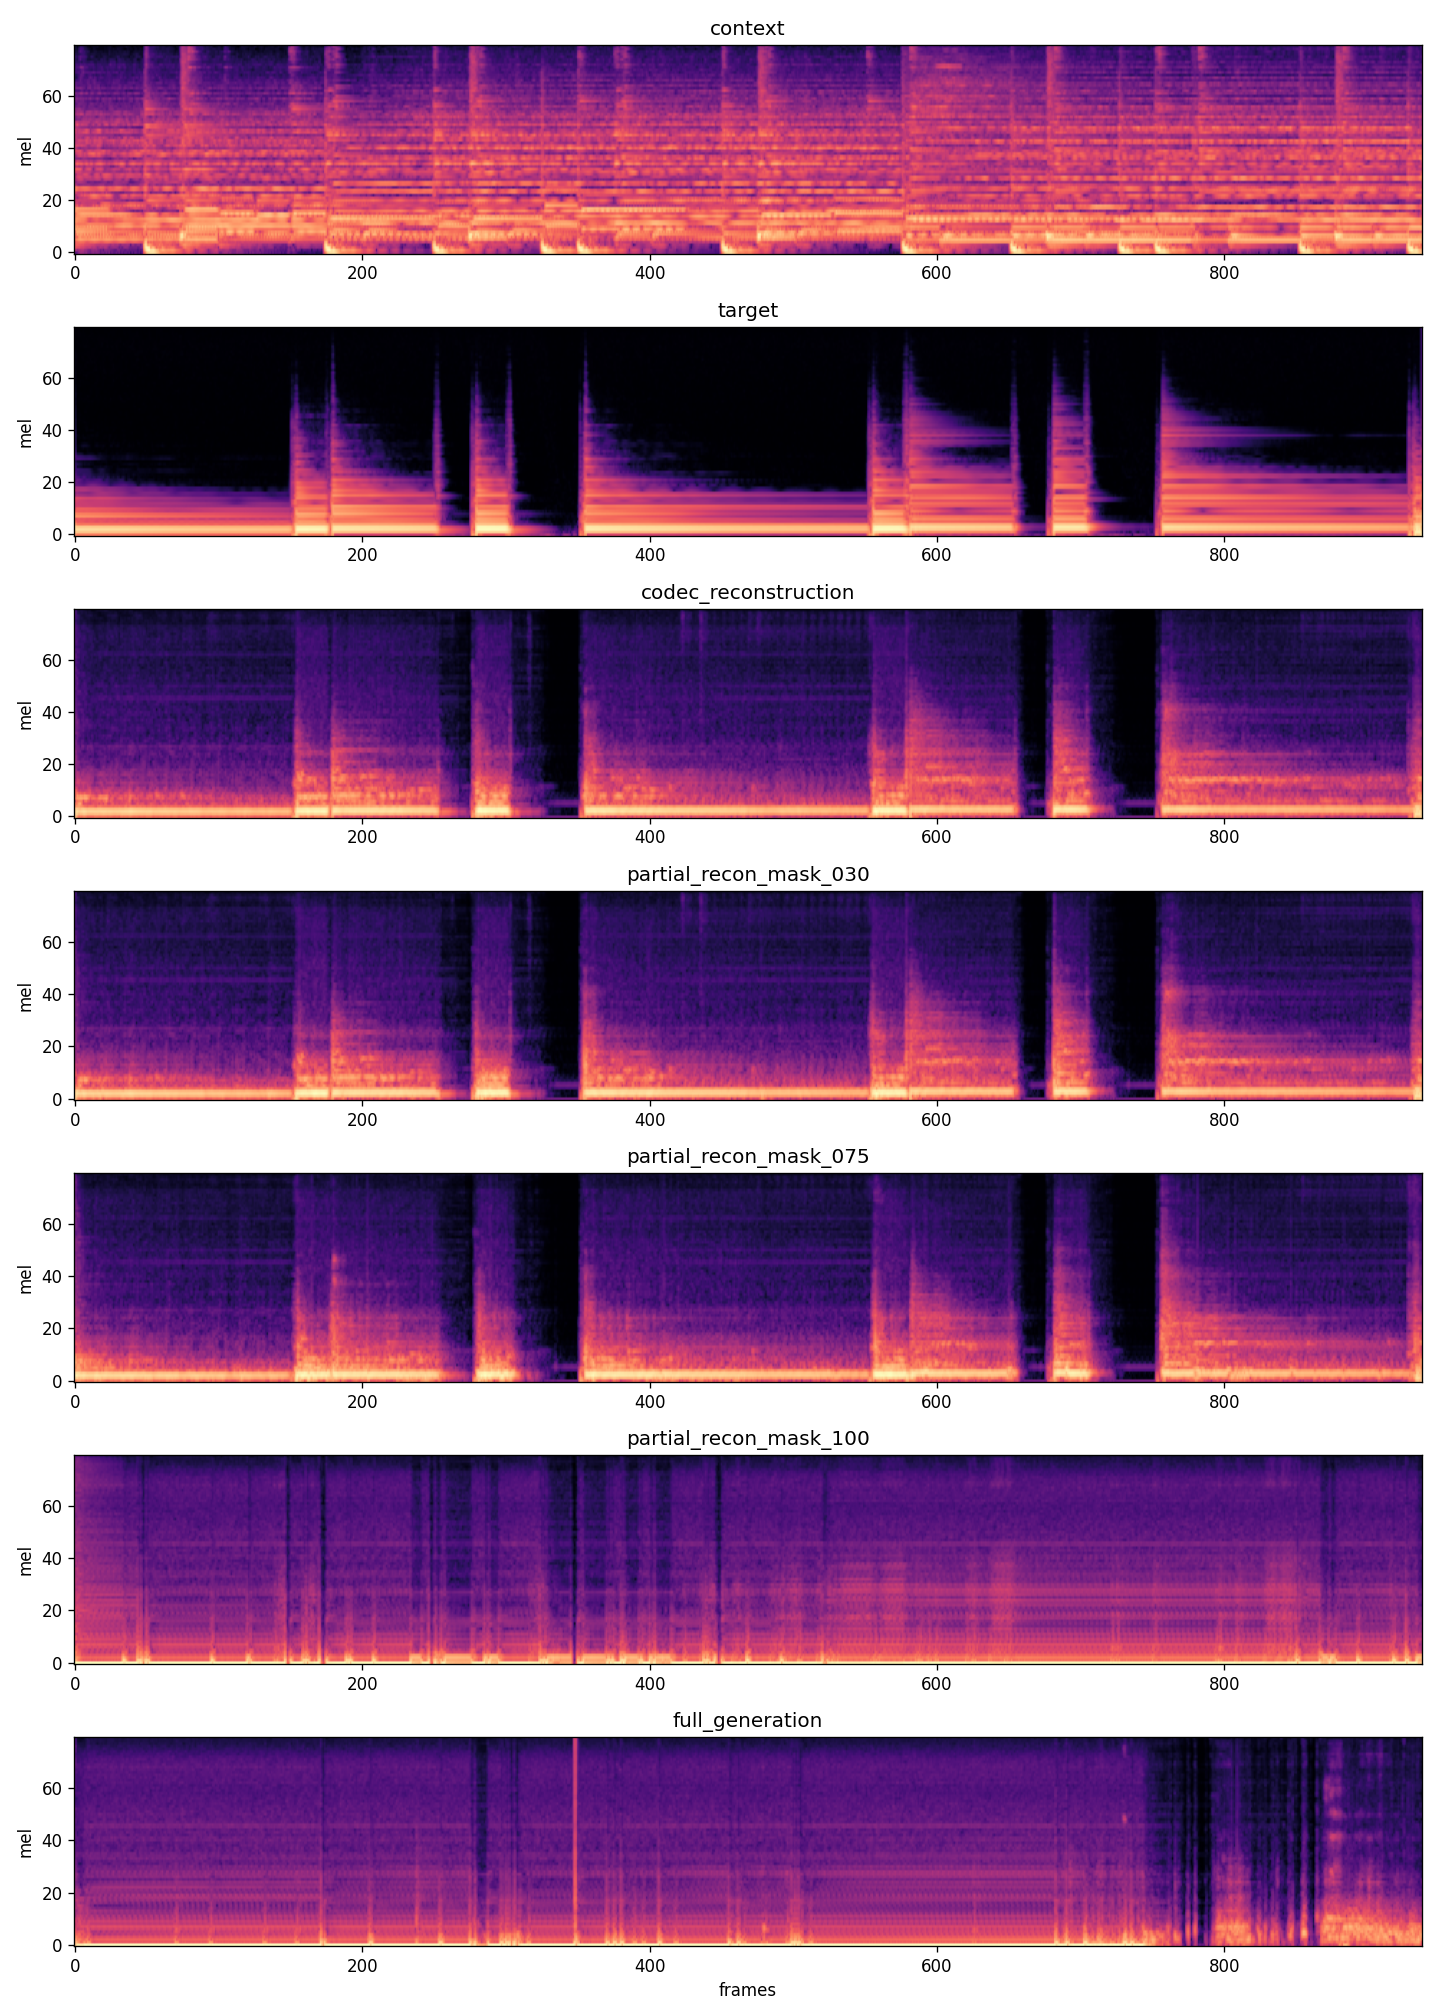
\includegraphics[width=\linewidth]{figures/diagnostic_mels_550.png}
    \caption{Mel-spectrogram diagnostic from a cached audio-token run. The important pattern is that codec and partial-mask reconstruction are more stable than full-mask generation.}
    \label{fig:mels}
\end{figure}

This result changes the interpretation of the project. The model is not simply broken: it learns useful conditional audio-token reconstruction. The remaining hard problem is generating all target tokens when no target information is visible.

The three diagnostic levels reveal different failure modes. In codec reconstruction, the spectrogram closely matches the ground-truth bass in both frequency content and temporal structure, confirming that the EnCodec tokenizer at 1.5 kbps with two codebooks is sufficient to represent bass at 24 kHz. In partial-mask reconstruction (50\% masked), the model correctly fills in missing segments that are consistent in pitch and energy with the visible surrounding tokens, indicating that the Transformer has learned local token-level statistics within a clip. In full 100\% mask generation, the generated spectrogram shows energy in the bass frequency range and some periodic structure, but the onset timing and harmonic content diverge from the target. This suggests the model has learned a prior over plausible bass textures but cannot reliably ground the generation in the specific context provided by the mixture.

The qualitative result also explains why validation accuracy alone can be optimistic. During training, the model often sees mask ratios below 100\%, so visible target tokens provide local rhythm and pitch hints. Full generation removes those hints entirely, requiring the model to infer a full bass line solely from the context mixture. This is the core difficulty of the StemGen task, and it is much harder than masked reconstruction. The failure mode is usually not silence: generated audio contains energy and some structure, but temporal alignment and spectral shape drift away from the target, which would be perceptually noticeable in a listening test.

\subsection{Audio-domain evaluation}

Token accuracy and mel diagnostics are useful but indirect. To measure quality in the audio domain, we ran \texttt{scripts/eval\_audio\_metrics.py} with the best 1000-track checkpoint on 20 held-out validation clips. The script decodes generated tokens to waveform and computes two metrics against the ground-truth bass: log-mel-spectrogram L2 distance (lower is better) and onset-alignment correlation between reference and generated onset-energy envelopes (higher is better, in $[-1,1]$). We evaluate the same three diagnostic levels used in the qualitative analysis.

\begin{table}[H]
\centering
\caption{Audio-domain metrics on 20 held-out validation clips. Values are mean $\pm$ standard deviation.}
\label{tab:audio_metrics}
\begin{tabular}{lcc}
\toprule
Level & Mel L2 distance $\downarrow$ & Onset score $\uparrow$ \\
\midrule
Codec reconstruction (ceiling) & $4.516 \pm 0.804$ & $0.608 \pm 0.166$ \\
Partial-mask reconstruction (50\%) & $4.746 \pm 0.855$ & $0.578 \pm 0.158$ \\
Full-mask generation & $19.280 \pm 5.944$ & $0.040 \pm 0.057$ \\
\bottomrule
\end{tabular}
\end{table}

The numbers in Table~\ref{tab:audio_metrics} support the qualitative result in Figure~\ref{fig:mels}. EnCodec reconstruction is a strong ceiling, so the tokenizer itself is not the main bottleneck. Partial-mask reconstruction stays close to that ceiling, which means the Transformer can repair missing token spans when local target context is available. Full-mask generation is much worse: the mel distance is about four times larger than the codec ceiling, and onset alignment is close to zero. This confirms that the remaining problem is not low-level decoding, but conditioning and global generation from mixture-minus-target context.

\subsection{MIDI branch baseline}

We also tested a symbolic MIDI route. The best frame-level activity result was HuBERT-mix with a GRU head, reaching 0.289 activity F1 on 200 tracks. CRNN-large with mix input reached 0.253 F1. A simple Transformer with mel/chroma features stayed around 0.11--0.13 F1. These results are much weaker than needed for complete stem generation, and they also move away from the StemGen audio-token formulation. Therefore, MIDI experiments are useful negative baselines but not the final method.

\subsection{Main lessons}

The experiments show three main lessons. First, data quality matters more than just the number of clips. The 1000-track run has fewer total clips than the 550 cached run, but it uses broader track coverage and lower-overlap fixed-stride windows. Second, codebook alignment is critical. If the codec, model, trainer, and generator disagree about codebook count, the decoded audio becomes unreliable. Third, full-mask generation is much harder than partial reconstruction. Future work should improve the decoding schedule, add condition dropout or classifier-free guidance, and train a larger model with a stronger tokenizer setting.

\section{Discussion}

The most important scientific finding is the gap between reconstruction and generation. Partial reconstruction asks the model to complete a damaged version of the true target. Full generation asks it to invent the whole bass stem from the mixture-minus-bass context. These are related but not the same problem. Our model is already useful for the first one, but still weak for the second one. This suggests that future training should put more pressure on full-mask or near-full-mask cases and should use decoding methods that better preserve long-range musical structure.

Another issue is the objective. Cross entropy treats every token error equally, but audio perception does not. A token mistake during an active bass note may be more important than a token mistake during a low-energy region. Also, two different token sequences can decode to similar audio. This makes token accuracy a useful debugging metric, but not a final music quality metric. A stronger evaluation should include mel distance, onset alignment, bass activity F1, and human listening comparisons.

The scale difference from the original StemGen paper is also large. The paper uses a much larger model and a stronger audio-token setup. Our model is intentionally small enough for a course project: 8 layers, 512 hidden size, two codebooks, and 10 second clips. Therefore, the fair conclusion is not that StemGen fails, but that a small reproduction can learn meaningful conditional token structure while still falling short on full stem synthesis. This is a useful outcome because it identifies the main bottleneck rather than only reporting a final demo.

If we continued the project, the next steps would be: train with more 100\% mask examples, add classifier-free guidance or condition dropout, compare different mask-predict schedules, add an activity-aware loss, and move from two to more codebooks only after increasing data and model capacity. We would also produce a small listening set with target, codec reconstruction, partial reconstruction, and full generation for the same examples, because that comparison is the clearest way to judge progress.

\section{Conclusion}

We completed a scaled-down but faithful reproduction of the StemGen audio-token idea. The final system converts context and target audio to EnCodec RVQ tokens, trains a masked-token Transformer with multi-codebook cross entropy, and uses iterative mask-predict decoding for bass stem generation. The best 1000-track fixed-stride cached run achieves 3.0279 validation loss and 0.572 validation token accuracy, clearly improving over earlier baselines.

The main limitation is full target generation from 100\% masking. Partial reconstruction is much stronger than full generation, which means the model has learned useful local audio-token structure but does not yet fully solve context-to-stem synthesis. Larger models, better mask schedules, stronger conditioning, and more codebooks are natural next steps.

\section{Code \& GitHub}

The project repository is:
\begin{center}
\url{https://github.com/daw041/ECE228_stemGen.git}
\end{center}
The repository includes training scripts, model code, data/config files, reproduction notes, presentation materials, and saved experiment logs. The main files are \texttt{src/model.py}, \texttt{src/codec.py}, \texttt{src/dataset.py}, \texttt{src/trainer.py}, \texttt{scripts/train.py}, \texttt{scripts/precompute\_audio\_token\_cache.py}, and \texttt{scripts/diagnose\_audio\_token.py}. The README gives setup, training, generation, and diagnostic commands.

\section{Team Member Contribution}

Dayong Wang mainly focused on the final report, while Youchen Qing mainly focused on the final presentation. Both members jointly read and discussed the StemGen paper, designed the audio-token reproduction plan, implemented and debugged the EnCodec tokenization pipeline, masked-token Transformer, trainer, and generation scripts, ran the Slakh data preparation and RunPod/H100 experiments, built the token-cache pipeline and MIDI baselines, and contributed to qualitative diagnostics and result analysis.


\begin{thebibliography}{9}

\bibitem[Copet et~al.(2023)]{musicgen}
Copet, J., Kreuk, F., Gat, I., Remez, T., Kant, D., Synnaeve, G., Adi, Y., and Defossez, A.
\newblock Simple and Controllable Music Generation.
\newblock \emph{NeurIPS}, 2023.

\bibitem[Defossez et~al.(2023)]{encodec}
Defossez, A., Copet, J., Synnaeve, G., and Adi, Y.
\newblock High Fidelity Neural Audio Compression.
\newblock \emph{Transactions on Machine Learning Research}, 2023.

\bibitem[Parker et~al.(2024)]{stemgen}
Parker, J. D., Spijkervet, J., Kosta, K., Yesiler, F., Kuznetsov, B., Wang, J.-C., Avent, M., Chen, J., and Le, D.
\newblock StemGen: A Music Generation Model That Listens.
\newblock \emph{ICASSP}, 2024.

\bibitem[Manilow et~al.(2019)]{slakh}
Manilow, E., Wichern, G., Seetharaman, P., and Le Roux, J.
\newblock Cutting Music Source Separation Some Slakh: A Dataset to Study the Impact of Training Data Quality and Quantity.
\newblock \emph{IEEE Workshop on Applications of Signal Processing to Audio and Acoustics (WASPAA)}, 2019.

\bibitem[Chang et~al.(2022)]{maskgit}
Chang, H., Zhang, H., Jiang, L., Liu, C., and Freeman, W. T.
\newblock MaskGIT: Masked Generative Image Transformer.
\newblock \emph{CVPR}, 2022.

\bibitem[Borsos et~al.(2023)]{soundstorm}
Borsos, Z., Sharifi, M., Vincent, D., et~al.
\newblock SoundStorm: Efficient Parallel Audio Generation.
\newblock \emph{arXiv preprint arXiv:2305.09636}, 2023.

\end{thebibliography}

\end{document}
